\subsection{Ловеринг операций и возможные стратегии}
\label{impl:lowering} % \index{Chapter8}

\newcommand{\divisible}{\mathop{\raisebox{-2pt}{\vdots}}}

Изучив особенности целевой архитектуры, перейдём к рассмотрению
конкретных стратегий ловеринга и их классификации. В связи с тем, что именно
работа с внешней память занимает большую часть времени, будем пытаться
оптимизировать еë. Как было упомянуто в одной из предыдущих глав, из-за малого
объëма внутренних кэшей данные приходится загружать частями, при этом каждая часть,
возможно, будет загружена несколько раз. В связи с этим, уменьшение количества
повторных загрузок --- самый простой способ оптимизации, а стратегия разбиения,
при которой достигается наименьшее количество повторных загрузок, будет считаться
нами наиболее оптимальной.

\subsubsection{Умножение матриц}

Умножение матриц в диалекте \texttt{ascend} представлено оператором \texttt{matmul}:

\begin{lstlisting}
func.func @kernel_func(
    %matrixA: memref<48x32x16x16xf16, 1>,
    %matrixB: memref<48x48x16x16xf16, 1>,
    %matrixC: memref<48x32x16x16xf16, 1>) {
    ascend.matmul(%matrixA, %matrixB, %matrixC) : memref<48x32x16x16xf16, 1>, memref<48x48x16x16xf16, 1>, memref<48x32x16x16xf16, 1>
    return
}
\end{lstlisting}

На вход оператор примает три многомерных массива, соответствующих матрицам
$A$, $B$, $C$ матричного умножения $C = A \times B$. Все три матрицы хранятся
в формате \texttt{Nz}, это сделано для удобства, т.~к. в реальных нейронных сетях
несколько умножений могут идти подряд, при этом результат предыдущего
передаётся на вход следующего. Привести кусок матрицы к необходимому формату
(\texttt{Zz} или \texttt{Zn}) не является проблемой при правильном использовании
операций копирования из GM в L1 и загрузки из L1 в L0. Число $1$ в конце каждого
\texttt{memref} означает, что массив находится в первом адресвом пространстве, что
соответствует памяти GM.

Теперь перейдём к тому, каким образом можно реализовать ловеринг и
оптимизировать количество копирований. Согласно статье FIXME, можно выделить
три основные стратегии: \textit{input stationary (IS)}, \textit{weight stationary (WS)}
и \textit{output stationary (OS)}. Отметим, что в данной статье рассматривается
операция свёртки, но всё перечисленное в ней верно и для умножения матриц.
Все три стратегии имеют общую идею: умножение производится блочно, блок одной из
матриц <<фиксируется>> ($A$ для IS, $B$ для WS и $C$ для OS), после чего
перебираются всевозможные блоки других матриц. Наглядное объяснение этого
процесса можно увидеть на картинке. После перебора выбирается другой блок и
операция повторяется.

\begin{figure}[h!]
    \centering
    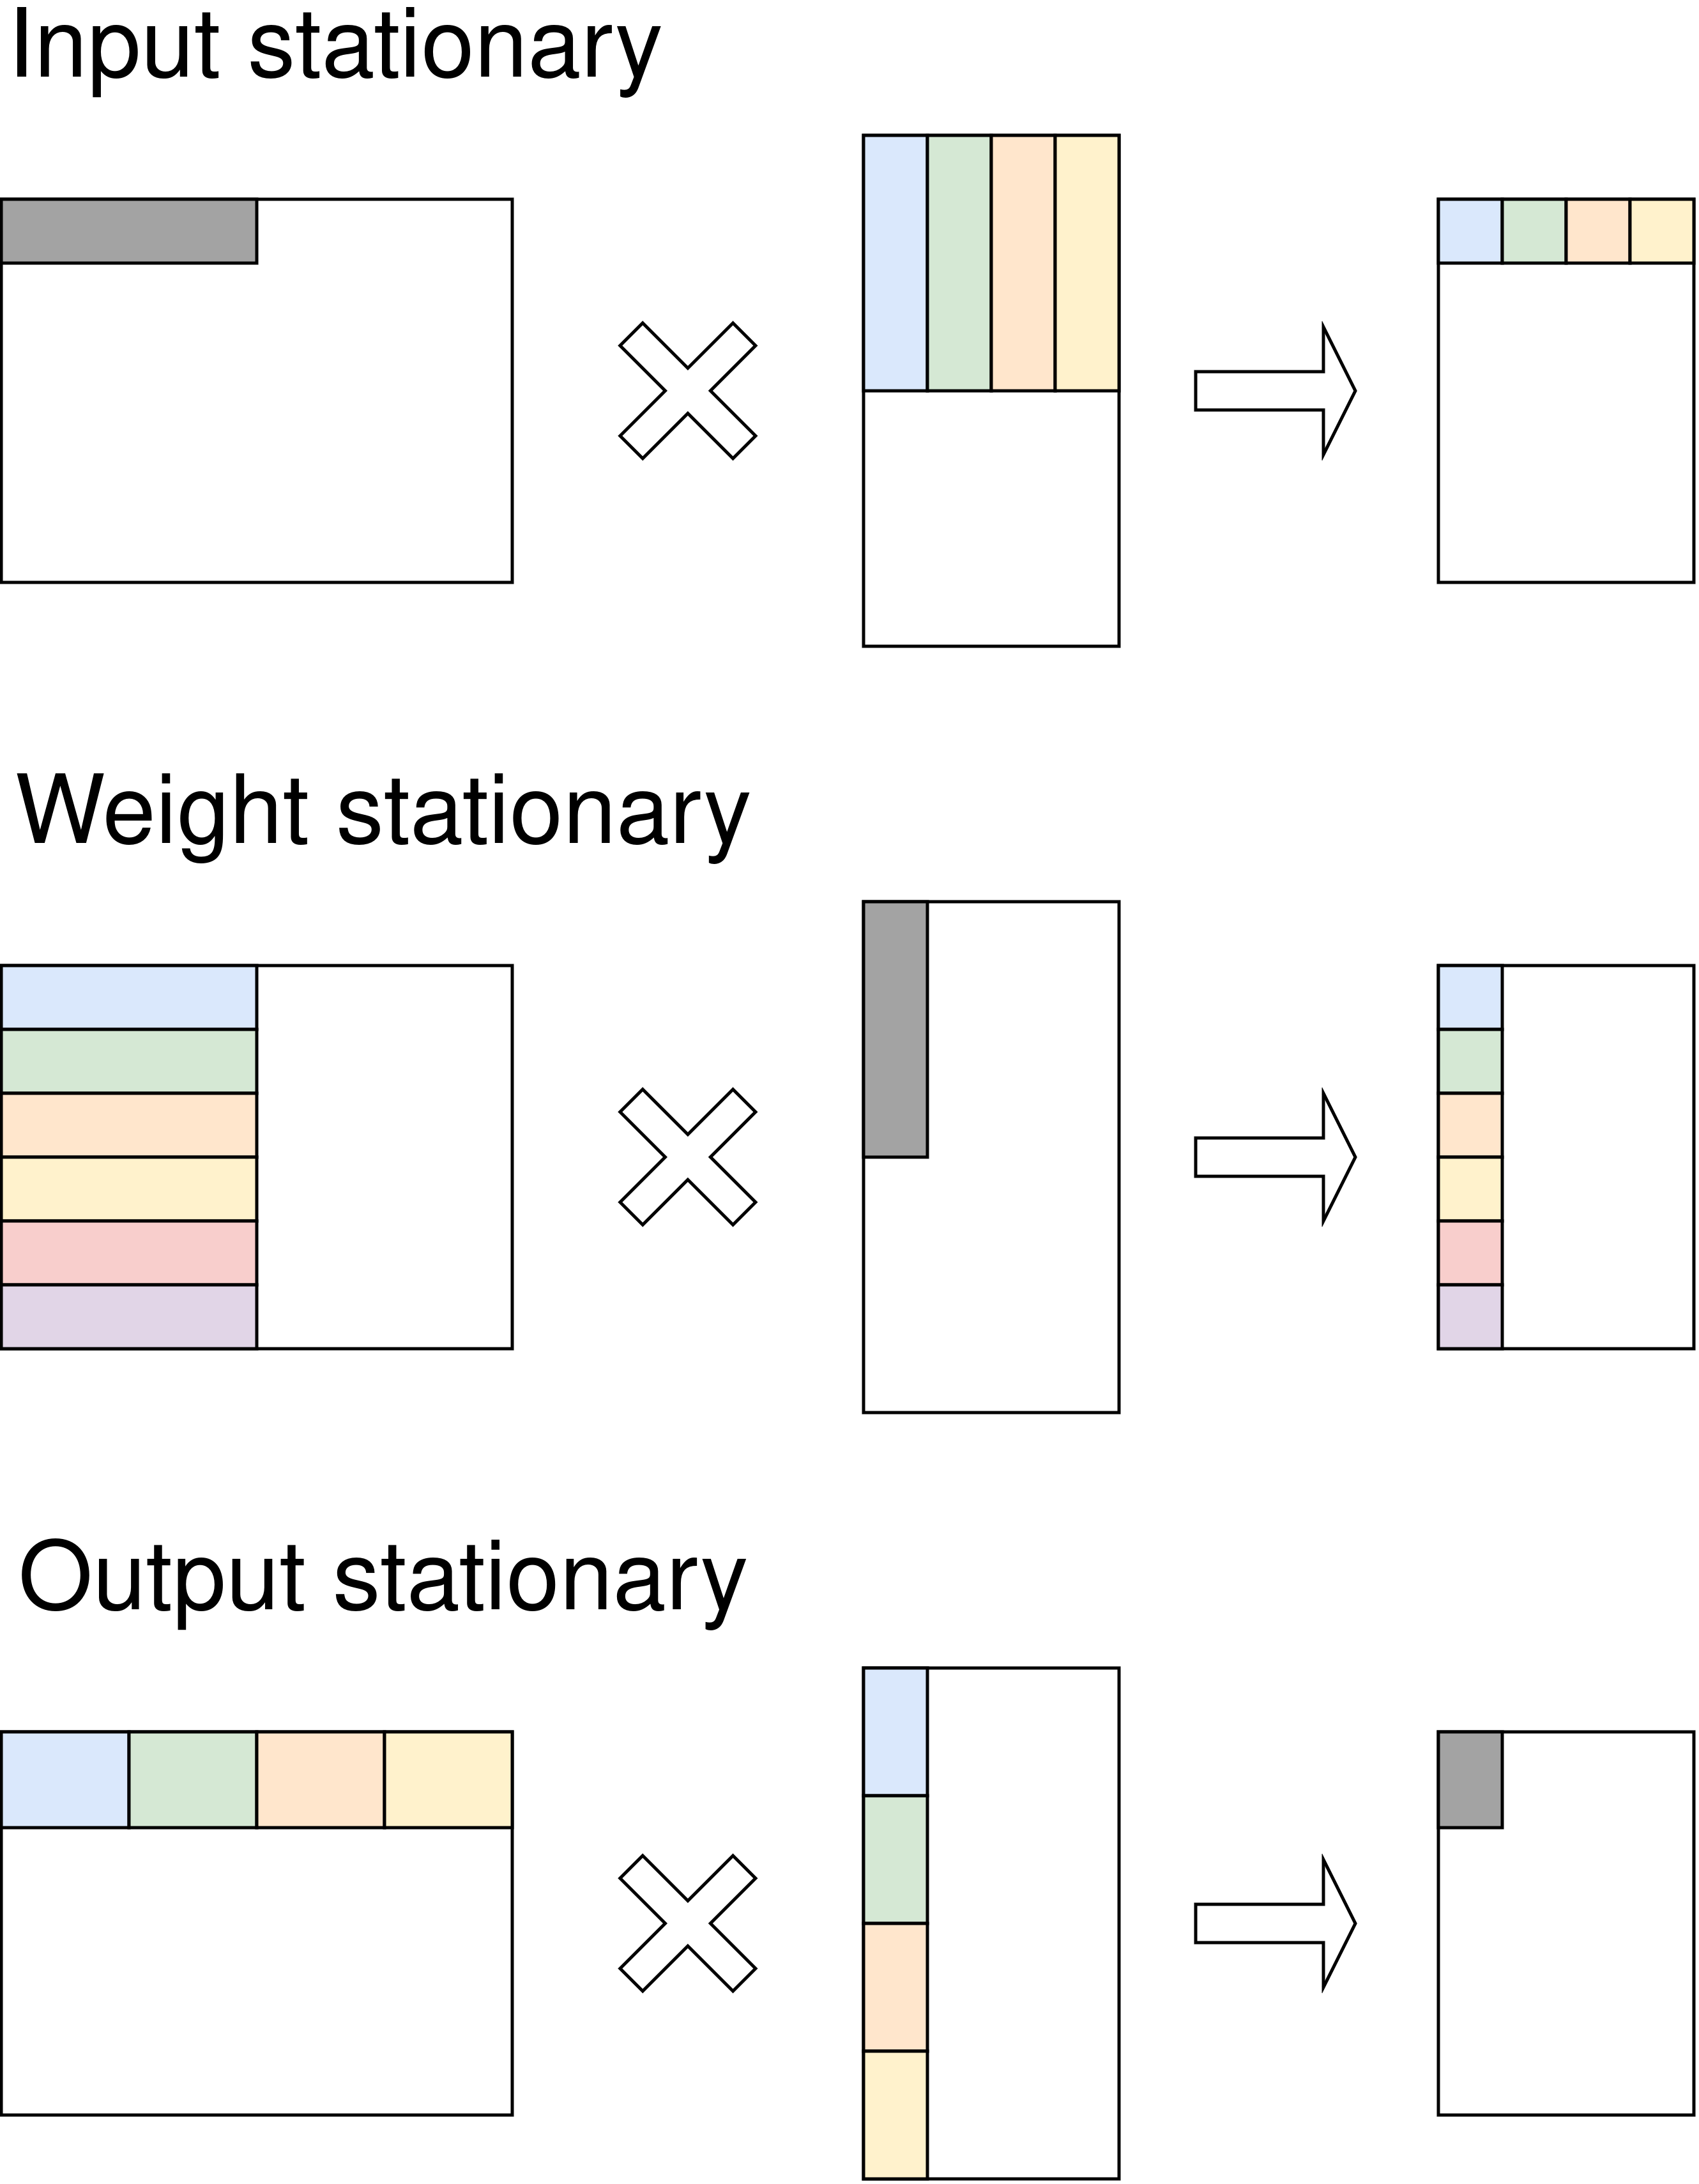
\includegraphics[scale=0.1]{Strategies.drawio.png}
    \caption{Стратегии для умножения матриц}
\end{figure}

Перечисленные стратегии описывают порядок обхода матриц по их блокам, но ничего
не говорят о размерах самих блоков. Пара стратегия + разбиение задаёт конкретное
исполнение, задача же состоит в том, чтобы выбрать конкретное исполнение, дающее
максимальную производительность. Для теоритического предсказания оптимального
исполнения нами была предложена метрика, соответствующая количеству загруженной
памяти. Опишем её более формально. Пусть матрица $A$ имеет размеры $M \times N$, а
матрица $B$ --- $N \times K$, тогда $C$ --- матрица $M \times K$. Таким образом,
матрицы описываются тройкой $(M, N, K)$. Аналогично, разбиение на блоки
описывается тройкой $(m, n, k)$. Будем рассматривать только такие конфигурации,
при которых блочное умножение можно выполнить за одну инструкцию, а выполнение
перебора блоков матриц при фиксации одного из них не требует выгрузки и загрузки
промежуточных результатов. В силу этих ограничений можно считать, что для IS
$k = K$ или $n = N$, а для WS --- $m = M$ или $n = N$.

Рассмотрим IS стратегию. Каждой загрузке матрицы $m \times n$ соответстует
$\frac{K}{k}$ загрузок матриц $n \times k$. Повторяется это действие
$\frac{MN}{mn}$ раз. Таким образом, общее количество загруженной памяти
составляет:

\[
    \Sigma_{IS} = \left( mn + nk ~ \frac{K}{k} \right) \frac{MN}{mn} = MN + \frac{MNK}{m}
\]

Аналогичным образом можно получить метрики для дугих стратегий:

\[
    \Sigma_{WS} = KN + \frac{MNK}{k}
\]

\[
    \Sigma_{OS} = MNK ~ \frac{m + k}{mk}
\]

На тройку $(m, n, k)$ должны быть наложены ограничения, связанные с размерами буферов.
Если считать, что элементы входных матриц имеют тип \texttt{float 16}, а выходной ---
\texttt{float 32} (это соответствует вычислениям на Ascend с повышенной точностью) тогда:

\[
\begin{cases}
    M, N, K, m, n, k \divisible 16 \\
    mn \leqslant 2^{15} \\
    nk \leqslant 2^{15} \\
    mk \leqslant 2^{16}
\end{cases}
\]

Итак, загружаемая память должна быть минимизирована, т.~е. $\Sigma \rightarrow \min$
Из эмпирических наблюдений (речь о которых пойдёт далее), при прочих равных используемая
память должна быть максимизирована:

\[
\begin{cases}
    mn \rightarrow \max \\
    nk \rightarrow \max \\
    mk \rightarrow \max
\end{cases}
\]

Для проверки гипотезы был разработан тестовый бенчмарк, замеряющий время
исполнения при различных конфигурацях. Гипотеза, изложенная выше, подтвердилась.
Если рассматривать типичные размеры умножаемых матриц в нейросетях (например,
BERT) --- $(512, 768, 768)$, то оказывается, что OS --- наиболее оптимальная
стратегия, а $(256, 128, 256)$ --- оптимальная конфигурация.

FIXME графики

OS стратегия была реализована в компиляторе на инфраструктуре MLIR в виде
понижения оператора \texttt{ascend.matmul} до цикла на диалектах \texttt{cce},
\texttt{affine} и \texttt{memref}. Ниже приведён псевдокод алгоритма:

\begin{lstlisting}
func ascend.matmul(matrixA, matrixB, matrixC) {
    for (x = [0, M / m)) {
        for (y = [0, K / k)) {
            c = empty_buf(m, k)
            for (sum_part = [0, N / n)) {
                a = empty_buf(m, n)
                b = empty_buf(n, k)
                load_part(a, matrixA, sum_part, y)
                load_part(b, matrixB, x, sum_part)
                cce.mad(a, b, c)
            }
            store_part(matrixC, c, x, y)
        }
    }
}
\end{lstlisting}

Подчеркнём, что в реальности алгоритм несколько отличается. Во-первых,
учитывается фрактализация матриц, их формат хранения. Во-вторых, операции,
названные в псевдокоде \texttt{load\_part} для $A$ и $B$ и \texttt{store\_part}
для $C$, состоят из двух этапов, для каждой матрицы по-разному:
$A: GM \rightarrow L1 \rightarrow L0A$, $B: GM \rightarrow L1 \rightarrow L0B$,
$C: L0C \rightarrow UB \rightarrow GM$. В-третьих, поддержана операция
\texttt{ascend.batch\_matmul}, которая производит умножение нескольких пар матриц
путём итерации по массивам пар.
